% Plan

% General intro into our motivations
% Lentilles gravitationelles
 %Brief history (Zwicky)
 %Modern motivation, data and other studies
 %Derivation of the main equations
% Interférométrie par masque non-régulier
 %Brief History
 %Moderne motivation, data and other studies
 %Derivation of main equations
% Inverse problem and Recurrent Inference Machine
 %General equation and motivation
 %Bayesian framework
 %RIM, what it solves -> implicit prior.


% Try doing without. Importantly, reader should not have to consult appendices to understand main text.
 %%Appendix for extended derivation of lens equation
 %%Appendix for angular diameter distance?
 %%Appendix for derivatives of likelihood for interferometry.
 %%Appendix on VAE
 
\chapter{Introduction}
\thispagestyle{empty}

% 1 ouverture -> les problèmes inverses, l'importance des images en astrophysique -> e.g. image des trou noirs de EHT.
% 2 sujet amené -> la reconstruction d'image dans le contexte de problèmes inverses
% 3 sujet posé -> La reconstruction d'image en astrophysique, deux cas d'études, les lentilles gravitationnelles et l'interférométrie par masque troué

%La recherche présentée dans ce mémoire s'intéresse au problème de reconstruction 
%d'image à partir de mesures incomplètes
%La recherche présentée dans ce mémoire approche le problème de cartographier la 
%masse gravitationnelle de galaxies-lentilles de façon agnostique. C'est-à-dire que 
%l'on ne suppose pas de modèle analytique simple pour résoudre le problème 
%de reconstruction non-linéaire et mal posé. Plutôt, cette recherche exploite 
%le cadre des machines à inférence récurrentielles (RIM) pour encoder des biais 
%inductifs dans un réseaux de neurones qui vont rendre l'inférence de 
%paramètres dans un espace à très haute dimension efficace et précise.

%Avant de décrire ce travail, je vais introduire les concepts 
%et les motivations nécessairent pour contextualiser ma recherche.
%En premier lieu, je vais décrire le concept de lentille 
%gravitationnelle à la section \ref{sec:lentilles gravitationnelles}. Ensuite, 
%je vais décrire quelque concepts lié à l'extraction de profiles de masses 
%provenant de large simulation magnétohydrodynamiques à la section 
%\ref{sec:simulation magnetohydrodynamique}. 
%Cette section sera suivit d'une introduction rapide à quelques concepts liés 
%à l'apprentissage machine utiles pour ma recherche
%à la section \ref{sec:apprentissage machine}. 
%Je vais décrire le formalisme bayesien pour les problème inverse 
%qui sous-tend ma recherche à la section \ref{sec:formalisme probleme inverse}.
%Finalement, je vais décrire 
%le contexte historique et scientifique qui motive ma recherche 
%à la section \ref{sec:contexte}.
%cadre plus large des motivations scientifiques 
%dans lequel cette recherche se situe à la section \ref{sec:motivations}.
%\citep{Morningstar2019

%A gravitational lens is composed of 
%massive objects ---or \textit{deflectors}--- in the line of sight that 
%magnify and distort luminous
%background objects like early-type star-forming galaxies \citep{Viera2013,Marrone2018,Rizzo2020,Sun2021},
%otherwise too faint to study with our 
%current ground and orbital telescope facilities. 
%This distortion is a very good tracer of mass, 
%independent of the electromagnetic 
%signature of the foreground deflector. As such, it 
%is one of the rare ways to study the 
%properties of dark matter 
%halos via its spatial distribution at the very small scales 
%\citep{Dala2002,Treu2004,Hezaveh2016,Gilman2020,Gilman2021}. 
%Gravitational lenses also act as cosmological rulers against which we can measure the 
%expansion rate of the universe by monitoring the flickering light of multiply imaged quasars 
%\citep[and reference therein]{Treu2016td,Millon2020} 
%or the dimming of multiply imaged supernovae \citep{Refsdal1964,Treu2016refsdal,Grillo2018}. 
%A central component of such cosmographic analysis is the 
%careful mass modelling of the lensing galaxy \citep{Chen2019,Wong2020} or 
%lensing galaxy clusters \citep{Kneib2011,Hoekstra2013,Natarajan2017,Bergamini2018,Jauzac2021}. 


%A common practice in galaxy mass modelling is to assume that the mass distribution of the 
%main deflector follows a power law $\rho \propto r^{-\gamma'}$ \citep{Keeton2001}.
%Following spectroscopic measurement 
%of the velocity dispersion of early-type galaxies, 
%a singular isothermal profile $\gamma' = 2$ can provide a good starting point for analysis
%\citep{Koopman2006,Barnabe2009,Auger2010}. For cosmographic measurments, 
%this assumption is relaxed by leaving the slope of the profile as 
%a free parameter in the mass modelling stage 
%since the isothermal approximation will induce a bias in the measurement 
%of the Hubble constant \citep{Treu2004,Birrer2020}. 
%Composite models can also be constructed as in \citet{Millon2020}, who 
%uses a Navarro-Frenk-White profile 
%\citep{Navarro1997} to model the dark matter halo that host the lensing galaxy 
%and a Sérsic profile \citep{Sersic1963} 
%to model the baryonic component of the galaxy. Even though these models 
%could produce a large range of profiles, best fit models often 
%have an average slope akin to an isothermal profile. This 
%observation is dubbed the \textit{bulge-halo conspiracy} \citep{Dutton2014}.

%Detailed modelling of high resolution images with high 
%signal-to-noise ratio (SNR) will additionally require external perturbations 
%to the main lensing galaxy coming from its local environment 
%\citep{Sluse2017,Wong2017,Birrer2019,Rusu2019} and 
%from the line of sight \citep{Rusu2017,Li2021} in order to fully capture the signal. 
%But, this approach becomes unwieldy as the quality of images increases. 
%More and more perturbations need to be added in order 
%to account for fine details in the data that are only revealed 
%in the high SNR regime. Famously,
%the Hubble Space Telescope (HST) Wide Field Camera 3 (WFC3) images of 
%the Cosmic Horseshoe (J1148+1930) --- initially discovered by \citet{Belokurov2007} --- 
%has many fine features that are hard to reproduce 
%\citep[e.g.][]{Bellagamba2016,Cheng2019,Schuldt2019}.



% rephrase
%Free-form methods --- also misleadingly called nonparametric ---
%attempt to relax the
%assumptions about the smoothness and symmetries of the mass distribution by 
%changing its parametric support. This includes regular (or adaptive)
%grid representations and meshfree representations
%\citep{Saha1997,Abdelsalam1998,Abdelsalam1998b,Diego2005,Birrer2015,Merten2016}. 
%These methods are more expressive and make better use of the information 
%contained in the arcs of the observed image in 
%order to constrain the mass distribution of the lens. 
%However, the widened range of distributions that can be represented 
%include non-physical solutions that must be penalized via regularization.
%% This is 
%% to say that strong inductive biases must be included during optimisation to 
%% exclude non-physical solutions from the parameter search. 

%% rephrase
%An important example is semi-linear inversion, originally 
%introduced by \citet{Warren2003} for grid-based source brightness reconstruction. 
%It was later improved to include 
%linear perturbation to the lensing potential \citep{Koopmans2005}. 
%The regularization procedure was also formalized into a Bayesian framework \citep{Suyu2006,Suyu2006b,Vegetti2009}, 
%such that it enabled detection of subhalos from distorted 
%Einstein rings or giant arcs \citep{Vegetti2010,Vegetti2012} 
%and constrain the subhalo mass function \citep{Vegetti2014,Li2016}. 
%This approach is generally limited to small perturbations from 
%the analytical profile used in a preliminary step to approximate the solution.
%As such, it is difficult to extend and automate this framework to reconstruct 
%lenses from hydrodynamical simulations.

%\citet{Morningstar2019} observed that the regularization employed in semi-linear inversion 
%only constrain a two-point prior, often resulting in noise leakage in the source 
%brightness distribution 
%due to the lack of knowledge on high order statistics. They showed that using a
%Recurrent Inference Machine \citep[RIM,][]{Putzky2017}, the neural network
%would implicitly incorporate a more complex prior from a dataset of galaxy images which 
%resulted in better performance overall for the background source reconstruction. 

%To learn such a machine, we turn to an optimisation problem 
%that is made feasible through the inductive biases
%introduced by
%\begin{enumerate}[label=(\subscript{\mathcal{H}}{{\arabic*}})]
	%\item \label{prior:architecture} The architecture of $G_{\varphi}$;
	%\item \label{prior:loss function} The loss function 
		%$\mathcal{L}: \mathcal{X}\times \mathcal{X} \rightarrow \mathbb{R}$.
%\end{enumerate}
%The feasibility of the optimisation problem is determined almost entirely 
%by the strength of these inductive biases. This follows from 
%the no-free lunch theorem for machine learning 
%\citep{Wolpert1995,Baxter2000}. The reader 
%might also refer to a modern discussion on inductive bias for machine learning 
%by \citep{Goyal2020} for review and insights. In the context of this work, 
%inductive biases can be defined as anything that might influence the 
%trajectory of the optimizer in $\varphi$-space during learning. 
%We attempt 
%to list them only in so far as they give a structure to our methods and 
%might give insights into our results.

%The no-free lunch theorem for machine learning \citep{Wolpert1995,Baxter2000} states 
%that strong inductive biases are the precondition to finding a solution 
%to an optimisation problem. This is particularly true for our case, 
%for which we know a general function $F^{-1}$ does not exist in the general sense. 
%However, we suspect that it is possible to find an inverse function when 
%the hypothesis space $\mathcal{H} \in \mathbb{H}$ is restricted enough 
%to exclude non-physical solutions.

%We describe the dataset in section \ref{sec:data}. 
%The model 
%architecture represents a family of functions with properties 
%that already encode some knowledge 
%about the model domain. For example, translational equivariance is built in 
%a convolutional neural network \citep[CNN, ][]{lecun1995}. This 
%manifests itself in the weight sharing and overall 
%reduced weight connectivity of CNN compared to fully connected network.
%Practitioners also 
%assume a certain locality to pixel covariance by using small convolution 
%kernels. These induction 
%biases makes CNN efficient
%and is one of the main reasons for their success in image recognition tasks
%\citep{Krizhevsky2012}.
%This was also clearly illustrated by \citet{Ulyanov2017}, who showed that a randomly initialized CNN in a U-net architecture \citep{Ronneberger2015}
%can learn the structure of natural images without the need for a training dataset. 
%In other words, the architecture can be thought of 
%as a form of implicit regularisation for certain problems. 


\section{Lentilles gravitationnelles de type galaxie-galaxie}\label{sec:lentilles gravitationnelles}
% Plan pour cette section: Dériver eq de la lentille et alpha
% Intro général: deflection de la lumière
%% Approcha a l'intro -> contexte historique à notre pensée sur la déviation de la lumière
%%% Réfraction 
%%%% Ptolémé (Optic, Grèce Antique)
%%%% Ibn Sahl (c. 940 - 1000)
%%%% Snell (1621)-Descartes(1637)
%%%% Principe de Fermat pour expliquer ce phénomène (lettre en 1657, mémoire en 1662)
%%%% Euler (1744) - Lagrange (1760) -> Principe de moindre action et sa solution
%%%% Équations de Maxwell (1861)

%%% déviation de la lumière par la gravité
%%%% Soldner, J. G. v. (1801–1804). "On the deflection of a light ray from its rectilinear motion, by the attraction of a celestial body at which it nearly passes by". Berliner Astronomisches Jahrbuch: 161–172.
%%%% Einstein 1911
%%%% Einstein 1915 (GR)
%%%% Eddington takes photograph of eclipse 1919
%%%% 1936 letter from Einstein at the request of 
%%%% Fritz Zwicky is first to postulate grav lensing idea in 1937i Zwicky, F. (1937) Nebulae as gravitational lenses. Physical Review, 51 (4). p. 290. ISSN 0031-899X
%%%% 1964 Refsdal (H0 and possibility to measure mass)
%%%%%% (Shapiro time delay (1964))
%%%% Fisrt gravitational lens discovered 1979 (double imaged quasar) https://www.nature.com/articles/279381a0
%%%% Then explosions of studies durings the 2000s on how to model things.

%%% Dark matter 
%%%% Zwicky 1933
%%%% Lambda CDM?
%%%% 

% Copied from https://royalsocietypublishing.org/doi/10.1098/rsta.2009.0209
%Henry Cavendish in 1784 is credited with the first (unpublished) calculation of the deflection angle 
%δ of a corpuscular light ray following a hyperbolic trajectory and the origin of the 
%(Newtonian) equation δ=2GM/Rc2. Subsequently, von Soldner (1804) published a similar calculation 
%deriving a deflection of 0.84 arcsec for stars viewed close to the limb of the Sun.

%Le principe de Fermat énonce que la trajectoire de la lumière, ou d'un 
%photon, doit suivre une trajectoire qui extrémise la durée de la trajectoire. 
%Ce principe mathématique, qui est un exemple du principe plus général de moindre action 
%développé par Lagrange en 1756, permet de décrire la trajectoire de la lumière 
%par l'entremise d'un simple indice $n$ (indice de réfraction) dans 
%lequel se cache toute la physique microscopique (ou macroscopique) 
%d'où émerge le phénomène qui nous intéresse. 


%L'expédition organisée par sir Arthur Eddington
%avait pour but d'observer 
%l'éclipse totale du 29 mai 1919 à partir de l'île de Prìncipe 
%dans le golfe de Guinée et de Sobral au nord du Brésil 
%\citep{Eddington1919}. Les photographes de l'éclipses prisent , bien qu'imprécises, 
%ont permis de valider la prédiction d'Einstein faite 
%en 1911 que la position observée d'une étoile serait déplacée de 
%$\delta \theta \approx 1.75'' \frac{R}{R_\odot}$ 
%durant une eclipse \citep{Dyson1920}, soit 2 fois plus 
%que ce qui est prédit par la théorie newtonienne.
%\subsection{Contexte historique}

Fritz \citet{Zwicky1937}, suivant les calculs publiés par \citet{Einstein1936}\footnote{Cacluls de Link} et la première observation 
de l'effet de déviation gravitationnelle de la lumière par \citet{Eddington1919}, 
est le premier à observer correctement qu'une lentille gravitationnelle 
est un objet particulièrement riche en information\footnote{On note l' existence de plusieurs travaux spéculatifs (et possiblement Link}. 
Ce phénomène se produit lorsque la lumière d'une source lointaine est fortement déviée par le champ gravitationnel d'un objet massif 
(e.g. une galaxie, un trou noir, une étoile, etc.) 
exceptionnellement bien aligné avec cette source selon le point de vue d'un observateur sur Terre.
L'article de \citet{Zwicky1937} articule précisément deux idées qui nous motivent encore aujourd'hui 
(plus de 85 ans plus tard) à étudier ces objets, soit
\begin{enumerate}
        \item d'imager des galaxies trop lointaine pour que l'on puisse les résoudre avec 
                nos télescopes;
        \item de mesurer directement la masse gravitationnelle de galaxies (appellées nébuleuse extra-galactique à l'époque) agissant 
                comme lentilles.
\end{enumerate}
\citet{Einstein1936} considérait l'éventualité d'observer ces systèmes extrêmement 
improbable en raison de la miniscule taille angulaire caractéristique d'un 
anneau d'Einstein-Chwolson \citep{Chwolson1924,Einstein1936}
\begin{equation}\label{eq:Taille Lentille}
        \theta_E \simeq 3\left( \frac{M}{M_{\odot}} \right)^{1/2} \left( \frac{D}{1\, \mathrm{Gpc}} \right)^{-1/2}\, \mu\mathrm{as} \hspace{1cm} \left\{D \equiv \frac{D_{\ell} D_s}{D_{\ell s}}\right\}\, .
\end{equation}
%À cette époque, la masses et la distances $D$ des nébuleuses extra-galactiques n'avaient pas de contraintes fiables\citep{Zwicky1937b}.
%Toutefois, même avec les suppositions les plus optimistes, la distance caractéristique entre deux images est attendu à être de 
%l'ordre de 1 seconde d'arc, une distance inférieur à la résolution des télèscopes optiques de l'époque (principalement 
%limité par les effets de turbulence de l'aire).

Dû à cette difficulté pratique, 
la première lentille gravitationnelle est découverte seulement $43$ ans après la prédiction de leur existence par \citet{Walsh1979}, 
suivant l'identification de deux spectres radios de quasars identiques, QSO 0957+561 A et B, séparés par seulement $5.7$ secondes d'arcs
et capturés avec le téléscope Mark II à l'observatioire Jodrell Bank. 
Les spectres partagent la même magnitude, $m=17$, le même décalage vers le rouge, $z=1.405$, et possèdent des détails 
chimiques suspicieusement semblables. Ces coïncidences suggèrent fortement que ces deux spectres sont deux copies provenant d'un même objet, soit un noyau 
actif d'une galaxie en arrière plan, produites par l'effet de lentille gravitationnelle d'une galaxie en avant plan, invisible dans le 
domaine radio à une fréquence de $966\,\mathrm{MHz}$. Cette hypothèse est rapidement confirmée par 
l'observation optique de la galaxie-lentille ($z=0.39$) avec l'observatoire Palomar \citep{Young1980}, simulténament 
observé et confirmé par le téléscope de $2.2\, m$ de l'Université d'Hawaii au mont Mauna Kea \citep{Stockton1980}, ainsi 
que la modélisation de sa distribution de masse, de son environnement 
et des angles de déflection qui causerait l'apparition d'une image double du quasar \citep{Young1981,Falc}
%par des modèles d'une complexité rapidement croissante suivant les observations subséquentes du 
%système \citep{Young1981}.
\begin{figure}[htb!]
        \centering
        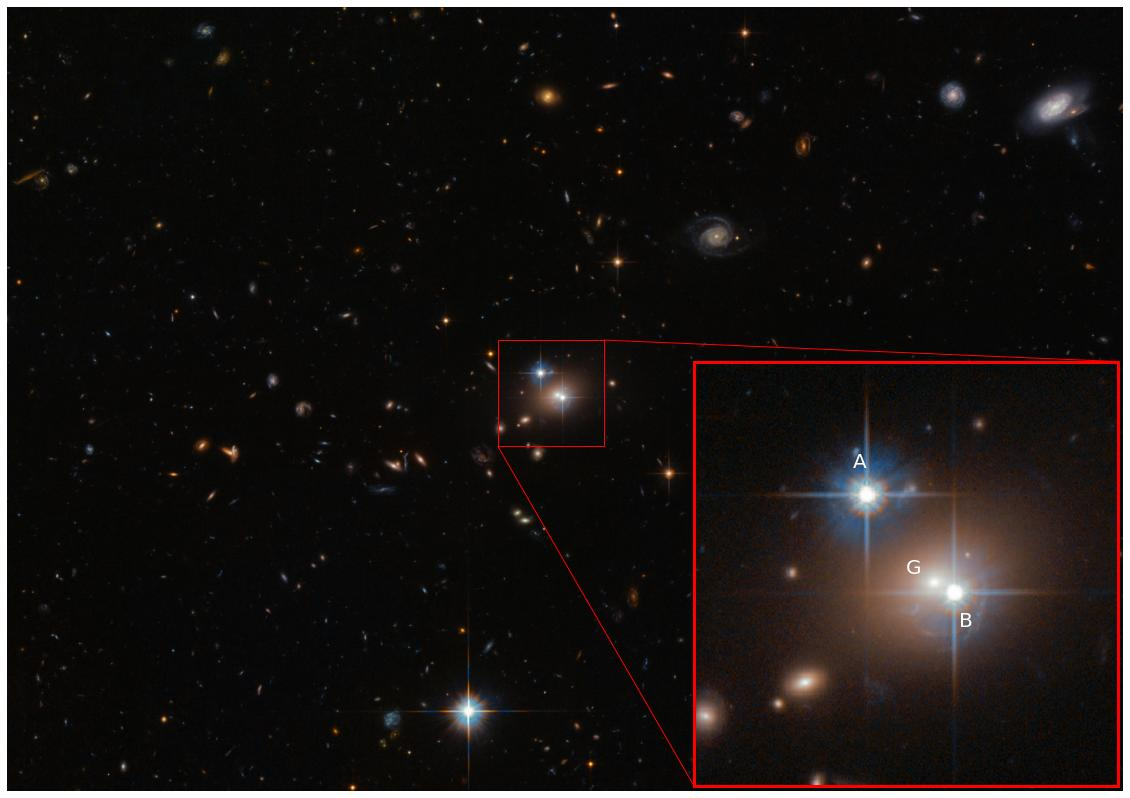
\includegraphics[width=0.8\textwidth]{figures/zoomed_in_qso0957}
        \caption{Le quasar double (QSO 0957+561 A et B) et la galaxie-lentille (G). Crédit: ESA/Hubble et NASA, enlargissement par AA.}
        \label{fig:doubel quasar}
\end{figure}

L'importance des lentilles gravitationnelles 
pour la cosmologie est subséquemment reconnue très tôt \citep[voir la revue de][]{Blandford1992}. Leur application dans 
ce domaine se divise principalement en 4 catégories:
%\begin{description}
        %\item{Cosmographie}
        %La cosmographie par délai temporelles \citep{Treu2016td,Suyu2017} permet, en particulier, de contraindre 
                %la constante de \citet{Hubble1929} $H_0$, mesurant le taux de l'expansion de l'Univers au temps présent. Les deux principales méthodes 
                %pour faire cette mesure sont la caractérisation de la courbe de lumière des supernovae \citet{Refsdal1964}, 
                %ç.-à-d. lentillé par une ou plusieurs galaxies \citep[e.g.][]{Kelly2015,Goobar2017}, et la surveillance décennale de quasars lentillés 
                %\citep[e.g.][]{Vanderriest1989,Wong2019};
%\end{description}
\begin{enumerate}
        \item La cosmographie par délai temporelles \citep{Treu2016td,Suyu2017} En particulier, le paramètre le mieux contraint est 
                la constante de \citet{Hubble1929} $H_0$, mesurant le taux de l'expansion de l'Univers au temps présent. Les deux principales méthodes 
                pour faire cette mesure sont la caractérisation de la courbe de lumière des supernovae \citet{Refsdal1964}, 
                ç.-à-d. lentillé par une ou plusieurs galaxies \citep[e.g.][]{Kelly2015,Goobar2017}, et la surveillance décennale de quasars lentillés 
                \citep[e.g.][]{Vanderriest1989,Wong2019};
        %\item Inférer la distribution de masse de la lentille pour une galaxie, ou un groupe de galaxie, et caractériser la distribution/présence 
                %de matière noire, voir même de trous noirs supermassif ou de planètes ou étoiles extragalactiques (tdcosmos);
%dark matter and its properties outside of the Milky Way \citep[e.g.,][]{Dala2002,Treu2004,Hezaveh2016,Gilman2020,Gilman2021}.
                % Microlensing 
        %\item De caractériser la structure de des protogalaxies dans l'Univers jeune, leur taux de formation d'étoiles et finalement 
                %imager directement le disque d'accrétion de trous noirs supermassifs, soit le noyau actif de galaxies dans l'Univers jeunes;
        %\item La recherche de plus de lentilles gravitationnelles et la caractérisation de leur propriétés de population pour l'inférence de 
                %de choses comme l'évolution des galaxies relié à leur contenu de matière noir, alpha, etc.
        
\end{enumerate}

%Cette découverte remarquable marque l'origine d'une ét
Le sujet de ce travail se concentre autour des lentilles gravitationnelles fortes de type galaxie-galaxie, e.g. QSO 0957+561. 
De tels systèmes sont caractérisé minimalement par une distortion de l'image source suffisamment forte pour causer 
l'apparition d'au moins deux images résolues de la source.
Pour une discussion plus général du phénomène, le lecteur peut se référer aux manuels de références par \citet{Meneghetti2013,Congdon2018} 
ou aux excellentes revues du sujet par \citet{Bartelmann2010,Treu2010}. 


%Une application importante de ces systèmes est l'étude du taux d'expansion de l'Univers 

%\subsection{Applications}
% Cosmologie - Image of RXJ1131 (mine) -> quasars
% Mass mapping + substructure detection (side mention of cluster and weak lensing) (constraints on dark matter?_
% Hierachecal studies (Ronan and previous paper Sonnenfeld etc)


%Il est intéressant de noter qu'\citet{Einstein1936} considérait la possibilité d'observer ce phénomène extrêmement improbable. En 
%fait, les calculs sont publiés 
%La résolution des télescopes optiques durant la majorité du XX\textsuperscript{e} siècle étaient 
%limités à environ $ 0.5$ arcsecondes par la turbulence de 
%l'air. Avec une telle résolution, un anneau d'Einstein d'une taille caractéristique de 1 arcseconde 
%apparaîtrait comme un point lumineux étalé, et ne serait donc pas distinguable d'une étoile. 

%Ce qu'il n'avait pas pris en compte c'est la possibilité de distinguer le spectre de l'objet 
%lentille à l'objet-lentille. En effet, comme ces objets se situent à deux redshift différent (pour un 
%système lentille observé en dehors du plan galactique de la Voie Lactée), alors il est possible en pratique 
%de détecter une lentille gravitationnelle simplement en analysant la raie spectrale du système. C'est de cette 
%façon que la première lentille gravitationelle fut découverte par \citet{Walsh1979} avec le téléscope radio Jodrell Bank MkIA. 
%Deux spectres identifiables à un rayonnement quasi-stellaire (quasar) presque identique, séparés de $5.7$ arcsecondes, 
%est la marque de la double image d'un seul quasar en arrière plan d'une galaxie. Dans ce cas particulier, le spectre de la 
%galaxie contamine légèrement le spectre de la contre-image du quasar, vu l'alignement imparfait. Il fallu quelques années 
%pour accepter ce résultat.

%Toutefois, cette première preuve expérimentale lanca le champ de recherche dans une nouvelle aire. L'étude du phénomène 
%s'est largement séparé en trois régime distinct: le régime micrométrique, le régime faible et le régime fort. Dans cette 
%étude, on s'intéresse principalement au régime fort, qui se distingue principalement des autres régime par le fait 
%que les déviations sont généralement de l'ordre de l'arcesecondes, de sortes qu'on peut observer les effet, et qu'on 
%distingue généralement plus d'une image de la source.

%Un autre direction de recherche, initiée par \citet{Refsdal1964}, est d'étudier l'évolution temporelle de supernovae lentillées 
%pour déterminer directement la constante de Hubble $H_0$, ou encore d'étudier, à une cadence de quelques jours entre chaque exposition, 
%un quasar lentillé plus d'une fois pour déterminer encore une fois la différence temporelle entre chaque image pour déterminer $H_0$.

%L'étude des effets de lentilles par les groups de galaxies est une discipline encore plus difficile que celle mentionnée jusqu'à maintenant, 
%dû à la complexité des profils de masses qui doivent être supposé et généralement dû à la difficulté de poser des contraintes qui requiert la mesure 
%de redshift de chaque images dans le champ de vue, et la présence de plusieurs sources différentes. On ne se concentre par sur cette étude, toutefois 
%on note que la recherche vers des algorithmes agnostiques sur le profil de marche est une avenue de recherche active dans cette discipline vu 
%la nécessité et aussi le genre de contraintes disponibles.

% Discovery of quasars in 1960
% First discovery of a grvaitational lens in 1979
% Explosion of their study -> models for the lens -> 2000s source reconstruction + H_0 motivations + cluster + others
% Saha 1997 first to try a full free-form reconstruction of galaxy-galaxy lens, his method has many limitations, requires strong regularisation and enormous hands-on fine-tuning 
% which makes the method hard to reuse / understand / caracterize its uncertainties
% Some free-form methods appear trying to correct error in the lensing potential of classical models for H_0. Then Birrer has his paper. 
% Explosion of machine learning in 2014. CNN are very efficient visual information processing tools. Laurence Yashar 2017
% Research in meta-learning lead to RIM (Putzky&Welling 2017), a general inverse problem solver that mimic traditional 
% gradient descent solver, but the prior is implicite, i.e. encoded as inductive biases in the neural network.
% Morningstar 2018/2019 use the method in the context of source reconstruction and interferometry reconstruction
% Our work.
% Context of our work
% Bulge-halo conspiracy, High SNR observation w/ JWST, Mass-sheet degeneracy?, Question is how to integrate information and use it properly
% Plan pour cette section: Dériver eq de la lentille et alpha
% Intro général: deflection de la lumière
%% Approcha a l'intro -> contexte historique à notre pensée sur la déviation de la lumière
%%% Réfraction 
%%%% Ptolémé (Optic, Grèce Antique)
%%%% Ibn Sahl (c. 940 - 1000)
%%%% Snell (1621)-Descartes(1637)
%%%% Principe de Fermat pour expliquer ce phénomène (lettre en 1657, mémoire en 1662)
%%%% Euler (1744) - Lagrange (1760) -> Principe de moindre action et sa solution
%%%% Équations de Maxwell (1861)

%%% déviation de la lumière par la gravité
%%%% Soldner, J. G. v. (1801–1804). "On the deflection of a light ray from its rectilinear motion, by the attraction of a celestial body at which it nearly passes by". Berliner Astronomisches Jahrbuch: 161–172.
%%%% Einstein 1911
%%%% Einstein 1915 (GR)
%%%% Eddington takes photograph of eclipse 1919
%%%% 1936 letter from Einstein at the request of 
%%%% Fritz Zwicky is first to postulate grav lensing idea in 1937i Zwicky, F. (1937) Nebulae as gravitational lenses. Physical Review, 51 (4). p. 290. ISSN 0031-899X
%%%% 1964 Refsdal (H0 and possibility to measure mass)
%%%%%% (Shapiro time delay (1964))
%%%% Fisrt gravitational lens discovered 1979 (double imaged quasar) https://www.nature.com/articles/279381a0
%%%% Then explosions of studies durings the 2000s on how to model things.

%%% Dark matter 
%%%% Zwicky 1933
%%%% Lambda CDM?
%%%% 

% Copied from https://royalsocietypublishing.org/doi/10.1098/rsta.2009.0209
%Henry Cavendish in 1784 is credited with the first (unpublished) calculation of the deflection angle 
%δ of a corpuscular light ray following a hyperbolic trajectory and the origin of the 
%(Newtonian) equation δ=2GM/Rc2. Subsequently, von Soldner (1804) published a similar calculation 
%deriving a deflection of 0.84 arcsec for stars viewed close to the limb of the Sun.

%Le principe de Fermat énonce que la trajectoire de la lumière, ou d'un 
%photon, doit suivre une trajectoire qui extrémise la durée de la trajectoire. 
%Ce principe mathématique, qui est un exemple du principe plus général de moindre action 
%développé par Lagrange en 1756, permet de décrire la trajectoire de la lumière 
%par l'entremise d'un simple indice $n$ (indice de réfraction) dans 
%lequel se cache toute la physique microscopique (ou macroscopique) 
%d'où émerge le phénomène qui nous intéresse. 


%L'expédition organisée par sir Arthur Eddington
%avait pour but d'observer 
%l'éclipse totale du 29 mai 1919 à partir de l'île de Prìncipe 
%dans le golfe de Guinée et de Sobral au nord du Brésil 
%\citep{Eddington1919}. Les photographes de l'éclipses prisent , bien qu'imprécises, 
%ont permis de valider la prédiction d'Einstein faite 
%en 1911 que la position observée d'une étoile serait déplacée de 
%$\delta \theta \approx 1.75'' \frac{R}{R_\odot}$ 
%durant une eclipse \citep{Dyson1920}, soit 2 fois plus 
%que ce qui est prédit par la théorie newtonienne.

%Dans l'intérêt de rendre ce manuscrit complet, je dérive à partir de principes 
%premier les deux équations centrales qui nous permettent 
%d'étudier les lentilles gravitationnelles.

\subsection{Les angles de déflections}
Dans les paragraphes qui suivent, je dérive les équations centrales qui nous permettent 
d'étudier les lentilles gravitationnelles de type galaxie-galaxie.
Mon traitement est largement inspiré 
des manuels de références de \citet{Meneghetti2013} et 
\citet{Carroll2003}.

Supposons qu'un photon est sur une trajectoire parallèle à l'axe de 
visée $\mathbf{e}_{\parallel}$ d'un observateur sur Terre. 
Supposons de plus que la source d'un champ gravitationnel $\Phi$ est situé sur l'axe de visée, 
ce qui a pour effet de courber la 
trajectoire de ce photon entre son point d'origine $A$ et son point d'arrivé $B$.
On définit l'angle de déviation comme la déviation totale de cette trajectoire 
dans la direction perpendiculaire à l'axe de visée de l'observateur. 
De façon générale, cette déviation s'écrit
\begin{equation}\label{eq:intro alpha}
        \boldsymbol{ \alpha} = - \int_{\lambda_A}^{\lambda_B} \ddot{\mathbf{x}} \times \mathbf{e}_{\parallel} d\lambda\, ,
\end{equation}
où $\lambda$ paramétrise la trajectoire du photon $\mathbf{x}(\lambda)$. 
Le signe négatif nous indique qu'on prend la perspective de l'observateur. 


%Pour résoudre l'intégrale \eqref{eq:intro alpha}, on doit déterminer la forme de 
%la trajectoire des photons dans un champ gravitationnel. Pour se faire, on faire usage du  
La trajectoire d'un photon est sujette au 
principe de Fermat, qui stipule que la lumière suit une trajectoire qui extrémise
la durée du parcours entre deux points. 
Dans le language du calcul 
des variations, la variation de la durée s'écrit
\begin{equation}\label{eq:Fermat}
        \delta T =  \delta \int_{A}^{B} n(\mathbf{x}(\ell)) \frac{d\ell}{c}= 0\, ,
\end{equation}
où $\ell$ est un élément de longueur sur la trajectoire et $n$ est un indice de réfraction.
Pour déterminer l'indice de réfraction du champ gravitationnel d'une galaxie, 
on doit utiliser le formalisme de la relativité générale. Selon le principe 
d'équivalence (fort), 
l'effet d'un champ gravitationnel est localement 
indistinguable d'une accélération causée par la courbure 
d'un espace-temps décrit par 
une métrique $g_{\mu \nu}$. 
La trajectoire d'un photon se trouve alors en cherchant 
les géodésiques de cet espace-temps. 
On fait l'approximation 
que le potentiel $\Phi$ d'une galaxie est celui d'un gas parfait, c'est-à-dire 
qu'il satisfait une équation de Poisson
\begin{equation}\label{eq:Poisson}
       \grad^{2}\Phi = 4\pi G \rho .
\end{equation} 
Dans la limite où ce potentiel est faible $\displaystyle \frac{2\Phi}{c^{2}} \ll 1$, la 
métrique $g_{\mu \nu}$ est décrite par une expansion au premier ordre autour de la 
métrique de Minkowsky %$\eta_{\mu\nu}$
\begin{equation}\label{eq:metrique}
        ds^2 = g_{\mu\nu}dx^{\mu}dx^{\nu} \approx \left( 1 + \frac{2\Phi}{c^{2}} \right)c^{2}dt^{2} - \left( 1 - \frac{2\Phi}{c^{2}} \right)d\mathbf{x}^{2}.
\end{equation} 
%Ici, j'ai choisit arbitrairement la signature $(+,-,-,-)$ pour la métrique.
Puisqu'un photon suit une géodésique de l'espace-temps $ds^{2} = 0$, on peut déterminer 
l'indice de réfraction en réarrangeant l'équation \eqref{eq:metrique}
\begin{equation}\label{eq:n}
        n \equiv c \left( \frac{\lVert d \mathbf{x} \rVert}{dt}  \right)^{-1} \approx  1 - \frac{2\Phi}{c^{2}}.
\end{equation} 
En réécrivant l'élément de longueur $d\ell$ en terme du 
paramètre de la trajectoire
$
        d\ell = \left\lVert\frac{d  \mathbf{x} }{d\lambda} \right\rVert d\lambda,
$
on peut réécrire l'équation \eqref{eq:Fermat} sous la forme
\begin{equation}\label{eq:Fermat2}
        \delta \int_{\lambda_A}^{\lambda_B} n(\mathbf{x}) \lVert \mathbf{\dot{x}} \rVert d\lambda = 0.
\end{equation} 
Par correspondance avec la fonctionnelle de l'action 
$J(x) = \int_{\lambda_0}^{\lambda_1} \mathcal{L}(\lambda,\, x,\,\dot{x}) d\lambda$ 
on trouve que 
le lagrangien de la trajectoire s'écrit 
$
        \mathcal{L} = n(\mathbf{x})  \sqrt{\dot{x}^{2}}.
$
La trajectoire qui satisfait \eqref{eq:Fermat} 
est une solution des équations d'Euler-Lagrange
\begin{equation}\label{eq:EulerLagrange}
        \frac{d }{d \lambda} \frac{\partial \mathcal{L}}{\partial \dot{\mathbf{x}}} - \frac{\partial \mathcal{L}}{\partial \mathbf{x}} = 0.
\end{equation} 
On a donc
\begin{equation}\label{eq:EulerLagrange2}
        \frac{d }{d \lambda} n \frac{\dot{\mathbf{x}}}{\lVert \dot{\mathbf{x}} \rVert}- \lVert \dot{\mathbf{x}} \rVert \grad n = 0 ,
\end{equation} 
Puisque le choix du paramètres $\lambda$ est libre, on peut le choisir tel 
que $\lVert \dot{\mathbf{x}} \rVert = 1$ en tout point de la trajectoire. Ainsi,
\begin{align}
        \nonumber
        \frac{d }{d \lambda} n \dot{\mathbf{x}} -  \grad n &= 0 \\
\label{eq:EulerLagrange3}
        \implies n \ddot{\mathbf{x}} + (\grad n \cdot \dot{\mathbf{x}}) \dot{\mathbf{x}} - \grad n &= 0
\end{align} 

À ce point de la dérivation, on utilise l'approximation de Born. 
C'est-à-dire qu'on approxime la trajectoire 
du photon comme une ligne droite sur l'axe de visée $\mathbf{e}_{\parallel}$. 
Cette approximation est justfiée 
dans le contexte des lentilles gravitationnelles de type galaxie-galaxie, 
puisque les angles de déviation sont généralement de 
l'ordre de l'arcseconde ou plus petit. 
Comme le vecteur $\dot{\mathbf{x}}$ est tangent à la trajectoire du photon, le 
terme $ \propto \dot{\mathbf{x}} \times \mathbf{e}_{\parallel} $ s'annule. 
En subsitutuant l'indice de réfraction par \eqref{eq:n} dans $\mathbf{e}_{\parallel} \times \eqref{eq:EulerLagrange3}$, on obtient
\begin{equation}\label{eq:sol}
        \ddot{\mathbf{x}} \times \mathbf{e}_{\parallel} = \frac{1}{n} \grad_\perp n = \grad_\perp \log n
        \approx -\frac{2}{c^{2}}\grad_{\perp} \Phi\,,
\end{equation} 
où $\grad_\perp$ est un gradient selon les coordonnées perpendiculaires à $\mathbf{e}_\parallel$.
On note que le facteur 2 qui apparaît dans l'équation \eqref{eq:sol} est un 
effet qui vient de la relativité générale. Ce facteur corrige la solution 
que l'on aurait obtenu avec une dérivation classique (newtonienne).


On est maintenant en mesure de calculer l'angle de déviation. 
J'introduit le paramètre d'impact $\boldsymbol{\xi}$ qui est la distance perpendiculaire entre 
la position d'origine du photon sur le plan de la lentille  
et l'axe de visé (voir Figure \ref{fig:cartoon}).
Dans le cas où le potentiel est généré par une masse $M$ ponctuelle, ç.-à-d.\ qu'on 
suppose $\rho = M\delta^{3}(\mathbf{x})$, où $\delta $ est la fonction delta de Dirac, 
alors le potentiel qui satisfait l'équation de Poisson \eqref{eq:Poisson} est 
la fonction de Green 
$\displaystyle \Phi = -\frac{GM}{\sqrt{ \xi^{2} + z^{2}}}$, où $z$ est la coordonné 
sur l'axe de visée. L'équation \eqref{eq:intro alpha} se réécrit finalement comme 
\begin{align}
\nonumber
        \boldsymbol{ \alpha}(\boldsymbol{ \xi} ) &= -\frac{2GM}{c^{2}} \int_{-\infty }^{\infty }  \frac{\partial}{\partial \boldsymbol{\xi} }\frac{1}{(\xi^{2} + z^{2})^{1/2}}dz \\
%\nonumber
        %&= \frac{2GM}{c^{2}} \boldsymbol{ \xi}  \int_{-\infty }^{\infty } \frac{1}{(\xi^{2} + z^{2})^{3/2}}dz  \\
\label{eq:deflection approx}
        \implies \boldsymbol{ \alpha}(\boldsymbol{ \xi})  &= \frac{4GM}{c^{2}  \xi^{2} } \boldsymbol{ \xi}
\end{align} 
Cette solution se généralise naturellement à un profil de masse quelconque en assumant 
qu'il s'exprime comme une somme d'élément de masses $dm = \Sigma d^{2}\boldsymbol{ \xi}'$, 
où $\Sigma = \int \rho dz$ est un densité surfacique de masse. 
L'angle de déviation total mesuré à un point $\boldsymbol{\xi} $ est alors une convolution 
sur tout le plan de la lentille (mince) puisque l'équation \eqref{eq:deflection approx} dépend 
linairement de la masse $M$:
\begin{equation}\label{eq:alpha physique}
        \boldsymbol{ \alpha} (\boldsymbol{ \xi} ) = \frac{4 G}{c^{2}} 
        \int_{\mathbb{R}^{2}} \Sigma (\boldsymbol{ \xi} ')
        \frac{\boldsymbol{ \xi}  - \boldsymbol{ \xi} '}{\lVert \boldsymbol{ \xi}  - \boldsymbol{ \xi} ' \rVert^{2}}d^{2}\boldsymbol{ \xi} '
\end{equation} 

L'angle de déviation est une quantité cruciale pour résoudre une lentille gravitationnelle 
puisqu'il décrit une transformation des coordonnées angulaires du plan de la lentille ($\boldsymbol{ \theta} $) 
vers les coordonnées angulaires du plan de la source ($\boldsymbol{ \beta} $). 
On assume que les distances entre l'observateur et la lentille $D_{\ell}$, entre l'observateur et la source $D_s$ et entre la lentille et la source $D_{\ell s}$, 
sont beaucoup plus grandes que les distances perpendiculaires à l'axe de visée $\boldsymbol{ \xi} $ ou $\boldsymbol{ \eta}$ 
(voir figure \ref{fig:cartoon}). 
Cette approximation est justifiée pour les objets qui nous intéresse,
pour lesquels les distances parallèles à l'axe de visée sont généralement 
de l'ordre du Gpc, alors que les distances perpendiculaire sont généralement 
de l'ordre du kpc; soit 6 ordres de grandeurs de différences.
Ainsi, on peut faire un argument géométrique (euclidien) 
\begin{align}
\nonumber
       D_{s} \boldsymbol{ \theta} &= \boldsymbol{ \eta}' \\   
\nonumber
       D_{s} \boldsymbol{ \beta} &= \boldsymbol{ \eta} \\   
\nonumber
       D_{\ell s} \boldsymbol{ \alpha} &= \boldsymbol{ \eta}' - \boldsymbol{ \eta}  \\   
\label{eq:lens equation}
       \implies D_s \boldsymbol{ \beta} &= D_s \boldsymbol{ \theta} - D_{\ell s} \boldsymbol{ \alpha}   
\end{align} 
La dernière relation est l'équation maîtresse qui nous permet de tracer les rayons lumineux d'une source 
vers un détecteur fictif dans nos simulations. On notera que cette relation reste valide pour un univers courbe et/ou en expansion 
(ç.-à-d.\ décrit par une géométrie non-euclidienne), 
à condition qu'on utilise une notion de distance qui satisfait, par définition, la relation trigonométrique euclidienne
\begin{equation}\label{eq:diameter angular distance}
       D \equiv \frac{\xi}{\theta}
\end{equation} 
%TODO finish this with a quick cosmological expression in an FRW universe. cite Dodelson and another manual for it

Il est généralement pratique de travailler avec la forme adimensionnelle de l'équation \eqref{eq:lens equation}. 
On introduit la densité critique 
\begin{equation}\label{eq:densite critique}
        \Sigma_c = \frac{c^2}{4 \pi G}\frac{D_{s}}{D_{\ell s} D_\ell}\, ,
\end{equation} 
qui nous permet de définir la quantité qu'on nomme convergence $\displaystyle \kappa(\boldsymbol{ \theta} ) \equiv \frac{\Sigma(\boldsymbol{ \theta})}{\Sigma_c}$. 
On définit ainsi l'angle réduit 
\begin{equation}\label{eq:alpha adim}
        \hat{\boldsymbol{ \alpha}} (\boldsymbol{ \theta}) = \frac{1}{\pi}\int_{\mathbb{R}^{2}} \kappa(\boldsymbol{ \theta} )
        \frac{\boldsymbol{ \theta} - \boldsymbol{ \theta}'  }{\lVert \boldsymbol{ \theta} - \boldsymbol{ \theta}' \rVert  } d^{2}\boldsymbol{ \theta}'\, ,
\end{equation} 
qui satisfait l'équation de la lentille adimensionnelle 
\begin{equation}\label{eq:lens equation adim}
        \boldsymbol{ \beta} = \boldsymbol{ \theta} - \hat{\boldsymbol{ \alpha}}(\boldsymbol{ \theta})\, . 
\end{equation}

\begin{figure}[H]
        \centering
        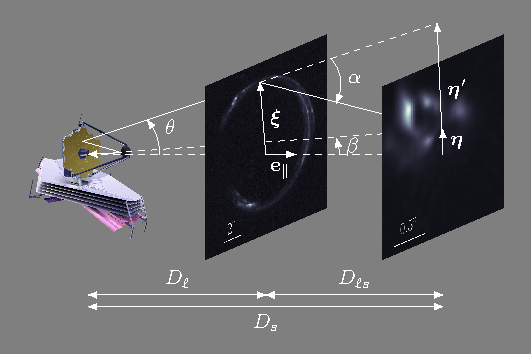
\includegraphics[width=0.8\textwidth]{figures/lensing_cartoon}
        \caption{Schéma d'une lentille gravitationnelle.}
        \label{fig:cartoon}
\end{figure}


% 




%Strong gravitational lensing is a natural phenomenon through which multiple distorted images of luminous background objects, 
%i.e. early-type star-forming galaxies, are formed by massive foreground objects along the line of sight 
%\citep[e.g.,][]{Viera2013,Marrone2018,Rizzo2020,Sun2021}. 
%These distortions are tracers of the distribution of mass in foreground objects, independent of the electromagnetic behaviour of these overdensities. 
%As such, this phenomenon offers a powerful probe of the distribution of 
%dark matter and its properties outside of the Milky Way \citep[e.g.,][]{Dala2002,Treu2004,Hezaveh2016,Gilman2020,Gilman2021}.

%Lens modeling is the process of inferring the parameters describing both the mass distribution in the 
%foreground lens and undistorted image of the background source.
%This has traditionally been a time- and resource-consuming procedure. 
%A common practice to model the mass of lensing galaxies is 
%to assume that their density profiles 
%follow simple parametric forms, e.g., a power law $\rho \propto r^{-\gamma'}$. 
%These profiles generally provide a good fit to low-resolution data and are easy to work with due to their small number of parameters \citep[e.g.,][]{Koopmans2006,Barnabe2009,Auger2010}. 
%However, as high-resolution and high signal-to-noise ratio (SNR) images become available, lens analysis with simple models requires the introduction of additional parameters representing the true complexity of the mass distribution in lensing galaxies and their immediate environments \citep[e.g.,][]{Sluse2017,Wong2017,Birrer2019,Rusu2019, Rusu2017,Li2021}. 
%This approach becomes intractable as the quality of images increases. For example,
%no simple parametric model of the Hubble Space Telescope (HST) Wide Field Camera 3 (WFC3) images of 
%the Cosmic Horseshoe (J1148+1930) --- initially discovered by \citet{Belokurov2007} --- 
%has been able to model the fine features of the extended arc 
%\citep[e.g., ][]{Bellagamba2016,James2018,Cheng2019,Schuldt2019}.

%Free-form methods --- also misleadingly called nonparametric methods ---
%attempt to relax the assumptions about the smoothness and symmetries of these parametric profiles 
%by changing their parametric support to more expressive families like regular (or adaptive)
%grid representations and meshfree representations. 
%But, this added flexibility comes at a price, which is (often) a high-dimensional inference problem that is under-constrained, meaning that imposing a prior on the reconstructed parameters becomes essential to penalize unphysical solutions and avoid overfitting the data. 
%% \citep{Bartelmann1996,Saha1997,Seitz1998,Abdelsalam1998,Abdelsalam1998b,Diego2005,Diego2007,Liesenborgs2006,Liesenborgs2007,Coe2008,Merten2009,Birrer2015,Merten2016,Torres-Ballestros2022}. 
% Kaiser And Squires Mass mapping weak lensing (leading up to Remy2022 - score based method reinforcing results from deep learning obtain 2 year prior by same group, and other method cited in this paper)
% Bartelmann 1996 (cluster lensing free-form reconstruction, with a priori known 10^5 galaxy source as background -> reconstruct potential starting from smoothed prior)
% Abdelsalam et al. (1998)
% Saha & Williams (1997)
% Seitz & Schneider (1998) Maximum entropy regularisation (cluster lensing, free-form inversion of the kappa map)
% Cacciato, Bartelmann 2006 -> combine weak and strong lensing info in cluster to reconstruct 2d potential, focus on using arcs to constrain the location of critical curves (very similar to Bradac work, except this critical curve thing)
% Jee et al 2007: Discovery of a ring-like dark matter structure in the cluster  Cl 0024+17 (pretty cool)
% Deb, Goldberg 2008: Particle Based Lensing, used for cluster reconstruction, can include all information like weak lensing, strong lensing constraints (image positions, flux, known position of critical curves)
% Liesenbourg (2006, -07, -09, -20): GRALE, genetic algorithm to infer kappa for cluster lensing by summing over basis function (Plummer profiles)
% Gosh et al 2020: GRALE can reconstruct cluster with up to 1000 multiple images for ultra deep fields images of certain clusters (e.g. w/ JWST)
% Diego et al 2005, 2007: WSLAP - probably the only method using pixel with no known arcs to constrain further the free-form mass model (mutliresolution grid parameter family)
% Bradac 2005a,b and 2009: SWUnited: combine weak and strong lensing info to break the mass sheet degeneracy for cluster lensing
% Coe et al 2008: LensPerfect - perfect reproduction of image position, flux and shear for cluster lenses. Explore thoroughly analytical priors for mass maps etc.
% Mertens 2009, -11, -16 SaWLens, 2009 explore the introduction of regularisation into the Weak + Strong lensing constraints, 2011: application to real data, 2016: mesh-free reconstructions.
%Free-form methods have a rich history in cluster-scale lensing \citep{Bartelmann1996,Seitz1998,Abdelsalam1998,Abdelsalam1998b,Bradac2005,Diego2005,Cacciato2006,Diego2007,Liesenborgs2006,Liesenborgs2007,Jee2007,Coe2008,Merten2009,Deb2012,Merten2016,Ghosh2020,Torres-Ballestros2022} and weak lensing \citep{Kaiser1993,Marshall2001,Massey2007,Deb2008,Simon2012,Leonard2012,Lanusse2016,Jeffrey2020,Starck2021,Remy2022}. They strive to make better use of the information contained in lensing features like resolved arc details, multiple image position, flux ratios, image deformation (i.e. weak lensing constraints) or even the null space of an image in order to place better constraints on the morphology of the mass density of the lens.
%On the other hand, comparatively less work has been done in the context of galaxy-galaxy lensing system to tackle free-form mass modelling directly \citep{Saha1997,Saha2004,Birrer2015,Coles2014}. The main reason for this state of affairs is the difficulty of specifying an appropriate prior which regularizes the problem over its non-linear parameters while maintaining computational tractability and sufficient flexibility to model a large variety of systems. 

% However, while these higher-dimensional parameter spaces add flexibility to the model, 
% exploring this complex multimodal space with traditional non-linear optimizers becomes quickly computationally intractable. 
% However, the price to pay for the flexibility of the free-form methods is (often) a high-dimensional inference problem that is under-constrained, meaning that imposing a prior on the reconstructed parameters becomes essential to penalize unphysical solutions and avoid overfitting the data. 

%In view of this, the focus of the field has instead been on using free-form methods for the background source reconstruction only. 
%A number of well-established procedures exists for linear inversion of pixellated-source models  in the context of traditional maximum likelihood modeling. These methods, originally developed by \citet{Warren2003,Suyu2006}, are based mainly on imposing a quadratic-log prior to the source pixels to regularize the optimisation. Subsequently, there have been multiple attempts at building a bridge toward free-form methods in order to correct simplistic assumptions on the mass density model by using linear corrections of the lensing potential \citep{Koopmans2005,Suyu2006b,Vegetti2009,Vegetti2012}, or iteratively specified priors for shapelets corrections \citep{Birrer2018,Nightingale2018}. But these extensions are generally limited by assumptions regarding the accuracy of the initial parametric models, and thus we are left wanting for a more flexible approach. 
% Despite this, the problem of developing a fully fledged method for a free-form mass density reconstruction algorithm in the context of galaxy-galaxy lensing remains open. 
% Many choices of priors are too constraining. overall this is a really hard problem, and it's so computationally expensive and degenerate that we can't test or characterize any of those models for systematics, let alone investigate ways correct for them.

%Over the recent years, deep learning methods have proven extremely successful at modeling quickly and accurately strong lensing systems \citep{Hezaveh2017,PerreaultLevasseur2017,Morningstar2018,Coogan2020,Park2021,Legin2021,Wagner-Carena2021,Schuldt2022,Wagner-Carena2022,Karchev2022,AnauMontel2022,Mishra-Sharma2022}.
%More specifically, \citet{Morningstar2019} demonstrated that recurrent convolutional neural networks can learn implicitly complex prior distributions from their training data to successfully reconstruct pixelated undistorted images of strongly lensed sources, circumventing the need to specify explicitly a prior distribution over those parameters. Motivated by this success, we propose a method that extends this framework to solve the full lensing problem and simultaneously reconstruct a pixelated lensing mass map and a pixelated undistorted background source.

%In this work, we propose a method for pixelated 
%strong gravitational lensing mass and source reconstruction, 
%allowing it to reconstruct complex distributions. 
%The method we propose here is based on the Recurrent Inference Machine (thereafter refered to as RIM), originally developed by \citet{Putzky2017}. 
%In this framework, we aim to learn an iterative inference algorithm, moving away 
%from hand-chosen inference algorithms and hand-crafted priors. 
%Instead, the prior is learned implicitly through the dataset used to train 
%the neural network that update the solution parameters at each iteration. 


\section{Interférométrie par masque non-régulier}

%\subsection{Contexte historique}

\subsection{Les angles de fermeture}

\subsection{Applications}


\section{Auto-encodeur variationnel}

\subsection{Description du modèle}

Les auto-encodeurs variationnels (VAE) ont été introduits par \citet{Kingma2013} comme une approche 
pour inférer approximativement les variables latentes (ou cachées) qui modélisent une distribution 
a posteriori définie implicitement via un échantillon de données. Dans cette section, j'introduis 
les concepts principaux relié à ce type de modélisation. 
Le lecteur peut aussi se référer au livre blanc de \citet{Kingma2019}.

On définit $\mathbf{z} \sim q(\mathbf{z})$ comme une variable latente et $\mathbf{x}$ comme un example d'un échantillon de donnée $\mathcal{D} = \{\mathbf{x}^{(i)}\}_{i=1}^{N}$. 
Notre objectif est de modéliser la distribution $p(\mathbf{x})$, implicitement décrite par notre échantillon. 
On suppose, sans perte de généralité, que la distribution de $\mathbf{x}$ fait partie d'une famille de distribution , caractérisé par $\theta$,  
conditionnelle à la variable cachée: $p_\theta(\mathbf{x \mid \mathbf{z}})$. 
Déterminer $p_\theta$ est généralement difficile, voir intraitable, si la dimensionalité de $\mathbf{x}$ est grande, ce qui est le cas 
pour des images pour lesquelles on trouve facilement $\mathrm{dim}(\mathbf{x}) > 10^{4}$. Pour résoudre cette difficulté, 
on introduit un modèle paramétrique d'inférence $q_\phi(\mathbf{z} \mid \mathbf{x})$ dont le rôle est de 
modéliser la distribution a posteriori de la variable latente pour la distribution qui nous intéresse
\begin{equation}\label{eq:vae 1}
        q_\phi (\mathbf{z} \mid \mathbf{x}) \approx p_\theta (\mathbf{z} \mid \mathbf{x})\, .
\end{equation} 
La notion de distance entre ces deux distributions est mesurée par la divergence de Kullback-Leibler $D_{\mathrm{KL}}(\cdot \KL \cdot) \geq 0$: 
\begin{align}
        \nonumber
       D_{\mathrm{KL}}(q_\phi(\mathbf{z} \mid \mathbf{x}) \KL  p_\theta (\mathbf{z} \mid \mathbf{x})) 
       &= \mathbb{E}_{q_\phi(\mathbf{z} \mid \mathbf{x})} \bigg[\log q_\phi(\mathbf{z} \mid \mathbf{x}) - \log p_\theta (\mathbf{z} \mid \mathbf{x}) \bigg]  \\
       \nonumber
       &= \mathbb{E}_{q_\phi(\mathbf{z} \mid \mathbf{x})} \bigg[\log q_\phi (\mathbf{z} \mid \mathbf{x}) -\log \frac{p_\theta(\mathbf{z}, \mathbf{x})}{p_\theta(\mathbf{x})} \bigg]  \\
       \label{eq:KL}
       &= \log p_\theta (\mathbf{x}) - \underbrace{\mathbb{E}_{q_\phi(\mathbf{z} \mid \mathbf{x})} \bigg[\log p_\theta(\mathbf{z}, \mathbf{x}) - \log q_\phi (\mathbf{z} \mid \mathbf{x}) \bigg]}_{\equiv \mathcal{L}_{\phi,\theta}(\mathbf{x})} \, .
\end{align} 

On remarque par cette manipulation que la distance $D_{\mathrm{KL}}$, en plus de mesurer la distance entre 
les deux distributions a posteriori (par définition), mesure aussi la différence entre le terme 
$\mathcal{L}_{\phi,\theta}(\mathbf{x})$, qu'on nomme limite inférieure sur l'évidence (de l'anglais 
\textit{evidence lower bound}: ELBO), et la distribution qui nous intéresse $p_\theta(\mathbf{x})$. 
L'objectif d'un modèle VAE est de maximiser la ELBO, $\mathcal{L_{\phi,\theta}}$. 
En observant l'équation \eqref{eq:KL}, on réalise que 
que ceci accomplit deux objectifs simultanément qui suivent du fait que la divergence KL est 
une quantité positive:
\begin{enumerate}
        \item Améliorer le processus génératif $p_\theta(\mathbf{x})$ puisque $\log p_\theta(\mathbf{x}) \geq \mathcal{L}_{\phi,\theta}(\mathbf{x})$;
        \item Améliorer le processus d'inférence puisque 
        $D_{\mathrm{KL}}(q_\phi(\mathbf{z} \mid \mathbf{x}) \KL  p_\theta (\mathbf{z} \mid \mathbf{x})) = \log p_\theta(\mathbf{x}) - \mathcal{L}_{\phi,\theta}(\mathbf{x})$ est simultanément minimisé.
\end{enumerate}

\begin{figure}[H]
        \centering
        \begin{tikzpicture}
                \node[circle, draw=black, minimum size=1cm] (z) at (0, 3) {$\mathbf{z}$};
                \node[circle, draw=black, minimum size=1cm] (x) at (0, 0) {$\mathbf{x}$};
                \draw[-{Latex[scale=2]}] (z) to (x);
                \draw[-{Latex[scale=2]}, in=225, out=135, dashed] (x) to (z);
                \node (phi) at (-2.5, 2.5) {$\phi$};
                \node (theta) at (2.5, 2.5) {$\theta$};
                \draw[rounded corners=0.5cm] (-1.5, -0.7) rectangle (1.5, 3.7);
                \draw[-{Latex[scale=2]}] (theta) to node[sloped, midway, below=5pt, fill=white, rectangle, draw=white, opacity=.8, text opacity=1] {$p_\theta(\mathbf{\mathbf{x} \mid \mathbf{z}})$} (x);
                \draw[-{Latex[scale=2]}] (theta) to node[sloped, midway, above=5pt, fill=white, rectangle, draw=white, opacity=.8, text opacity=1] {$p_\theta(\mathbf{z})$} (z);
                \draw[-{Latex[scale=2]}, dashed] (phi) to node[sloped, midway, above=5pt, fill=white, rectangle, draw=white, opacity=.8, text opacity=1] {$q_\phi(\mathbf{z} \mid \mathbf{x})$} (z); 
                \node at (1, -0.5) {$N$};
        \end{tikzpicture}
        \caption{Modèle graphique d'un VAE. Les flèches pleines indiquent le processus génératif, alors que les flèches pointillées indiquent le processus d'inférence.}
        \label{fig:vae encoder}
\end{figure}

\subsection{Le truc de reparamétrisation}
Le gradient de la ELBO par rapport aux paramètres variationnels, $\grad_{\phi,\theta}\mathcal{L}_{\phi,\theta}(\mathbf{x})$, 
est une quantité qu'on doit calculer pour faire usage d'algorithmes comme la grimpe de gradient stochastique 
pour maximiser la ELBO en terme de $\phi$ et $\theta$. 
Or, la liste de paramètres $\phi$ apparait dans la distribution de prélevement pour calculer 
l'espérance mathématique $\mathbb{E}_{q_\phi(\mathbf{z} \mid \mathbf{x})}$ dans la ELBO \eqref{eq:KL}.
Cette opération n'a pas de dérivée formelle en terme de $\phi$. 

Pour résoudre ce problème, on utilise le truc de reparamétrisation \citep{Kingma2013}, 
qui consiste à restreindre la forme fonctionnelle de $q_\phi(\mathbf{z} \mid \mathbf{x})$ à une famille paramétrique 
qui s'exprime comme la transformation différentiable d'une variable aléatoire auxiliaire $\boldsymbol{ \epsilon}$. 
On considère le cas où $q_\phi(\mathbf{z} \mid \mathbf{x})$ et $p(\boldsymbol{ \epsilon})$ 
font partie de la famille gaussienne isotropique
\begin{align}
        \label{eq:p epsilon}
        p(\boldsymbol{\epsilon}) &\equiv \mathcal{N}(0, \bbone)\, ;\\
        \label{eq:q phi}
        q_\phi(\mathbf{z} \mid \mathbf{x}) &= \mathcal{N}(\boldsymbol{ \mu}_\phi (\mathbf{x}),\, \bbone e^{\log \boldsymbol{\sigma}_\phi^{2}(\mathbf{x})})\, ;\\
        \label{eq:reparametrisation}
        \mathbf{z} &= \boldsymbol{\mu}_\phi + \boldsymbol{ \sigma}_\phi \odot \boldsymbol{ \epsilon}\, .
\end{align} 
$\odot$ symbolise le produit d'Hadamard, ou encore le produit élément-par-élément de vecteurs.
La reparamétrisation fait en sortes que les paramètres variationnelles ne participent plus au procsessus de prélevement, 
maintenant pris en charge par $\boldsymbol{ \epsilon} $. Cette propriété est cruciale 
dans le but de prendre le gradient de la ELBO \eqref{eq:KL}. 
En effet, on peut maintenant échanger les opérateurs $\grad_{\phi,\theta}$ et ${\mathbb{E}_{q_\phi(\mathbf{z} \mid \mathbf{x})} = \mathbb{E}_{p(\boldsymbol{ \epsilon})}}$,
ce qui nous permet d'appliquer le gradient à l'intérieur de l'espérance mathématique.
De plus, $\phi$ décrit maintenant une fonction générique dont le rôle est d'inférer les 
paramètres d'une distribution gaussienne isotropique \eqref{eq:q phi}, ${f_\phi(\mathbf{x}) = (\boldsymbol{\mu}, \log \boldsymbol{\sigma}^{2})}$, 
étant donné la valeure d'un échantillon $\mathbf{x}$. En pratique, on peut construire une approximation de 
cette fonction avec un réseau de neuronnes convolutionnelles. 

Pour déterminer la forme fonctionnelle de la ELBO, on stipule a priori que la distribution marginale des variables latentes 
devrait correspondre à une distribution normale isotropique
\begin{equation}\label{eq:latent distribution}
        p_{\theta}(\mathbf{z}) = \mathcal{N}(0, \bbone)
\end{equation}
On est libre de faire ce choix sans pour autant limiter les formes possibles de la distribution qui nous intéresse $p_\theta(\mathbf{x})$.
On peut alors exprimer la ELBO comme
\begin{align}
        \mathcal{L}_{\phi,\theta}(\mathbf{x}) &= \mathbb{E}_{q_\phi(\mathbf{z} \mid \mathbf{x})} \bigg[ \log p_\theta(\mathbf{z}, \mathbf{x}) - \log q_\phi (\mathbf{z} \mid \mathbf{x}) \bigg]\, ; \\
        \label{eq:final elbo}
         \implies \mathcal{L}_{\phi,\theta}(\mathbf{x})  &= 
         \underbrace{\mathbb{E}_{q_\phi(\mathbf{z} \mid \mathbf{x})} \bigg[ \log p_\theta(\mathbf{x} \mid \mathbf{z})\bigg]}_{\text{terme de reconstruction}}
         + \underbrace{
                \mathbb{E}_{q_\phi(\mathbf{z} \mid \mathbf{x})} \bigg[\log p_{\theta}(\mathbf{z}) - \log q_\phi (\mathbf{z} \mid \mathbf{x}) \bigg]
        }_{\equiv -D_{\mathrm{KL}}(q_\phi(\mathbf{z} \mid \mathbf{x})\, \KL\, p_\theta(\mathbf{z}))}\, .
\end{align} 
La divergence de KL obtenue au second terme du membre droit de l'équation \eqref{eq:final elbo} 
admet une solution fermée étant donné les familles paramétriques stipulées 
pour $p_\theta(\mathbf{z})$ \eqref{eq:latent distribution} et $q_\phi(\mathbf{z} \mid \mathbf{x})$ \eqref{eq:q phi}
\begin{equation}\label{eq:}
        -D_{\mathrm{KL}}(q_\phi(\mathbf{z} \mid \mathbf{x})\, \KL\, p_\theta(\mathbf{z})) =
        \frac{1}{2}\sum_{j=1}^{\mathrm{dim}(\mathbf{z})} (1 + [\log \boldsymbol{ \sigma}_\phi^{2} ]_j - [\boldsymbol{ \mu}_\phi ]_j - [\boldsymbol{ \sigma}_\phi^{2} ]_j)
\end{equation} 
Une dérivation de ce terme est donnée dans l'appendice B de \citet{Kingma2013}. 
%Cette solution se dérive directement par rapport à $\phi$. 
Le premier terme du membre droit de l'équation \eqref{eq:final elbo} 
est nommé \textit{terme de reconstruction} puisqu'il connecte avec l'objectif des fonctions 
de type auto-encodeurs d'apprendre une représentation latente d'un échantillon de données.
La reconstruction s'accomplit en utilisant d'abord le modèle d'inférence $\mathbf{z}^{(1:L)} \overset{\mathrm{i.i.d}}{\sim} q_\phi(\mathbf{z} \mid \mathbf{x})$\footnote{
$\mathrm{i.i.d}$: identiquement et indépendamment distribué.}
pour obtenir un échantillon de représentations latentes à partir des équations \eqref{eq:p epsilon} à \eqref{eq:reparametrisation}, 
puis en utilisant le modèle génératif $\hat{\mathbf{x}}^{(i)} \sim p_\theta(\mathbf{x} \mid \mathbf{z}^{(i)})$ pour obtenir 
un échantillon de reconstructions $\mathbf{\hat{x}}^{(1:L)}$ similaire à l'exemple originel $\mathbf{\mathbf{x}}$. 
Comme on a déjà une variable auxiliaire $\boldsymbol{ \epsilon} $ 
qui se charge de l'aspect génératif du modèle, on peut construire une approximation du 
modèle génératif avec une fonction générique des variables latentes 
$g_\theta(\mathbf{z}^{(i)}) = \hat{\mathbf{x}}^{(i)}$. Encore une fois, un réseau de neuronnes convolutionnelles est un choix pratique pour modéliser cette fonction 
dans le cas où $\mathbf{x}$ est une image. En général, on choisit une erreur quadratique moyenne pour modéliser le terme de reconstruction, 
de sorte que
\begin{equation}\label{eq:reconstruction}
        \mathbb{E}_{q_\phi(\mathbf{z} \mid \mathbf{x})} \bigg[
                \log p_\theta(\mathbf{x} \mid \mathbf{z})
        \bigg] 
        \simeq -\frac{1}{L}\sum_{i=1}^{L} \lVert \mathbf{x} - \hat{\mathbf{x}}^{(i)} \rVert_2^{2}
\end{equation} 

Je note que la fondation théorique des auto-encodeurs variationnels repose sur le principe plus général 
du goulot d'information \citep{Tishby1999}; un sujet qui n'est pas abordé dans ce travail, mais qui motive 
l'utilisation de la version $\beta$-VAE du modèle esquissé dans cette section. Sans rentrer dans les détails, on note 
qu'il est possible de dériver l'objectif de notre auto-encodeur via la théorie de l'information de \citet{Shannon1948} en interprétant 
l'auto-encodeur comme un système de transmission d'information par compression, avec perte. 
Une approche naïve pour modéliser ce système serait de maximiser le taux d'information transmise par le système, 
ç.-à-d. que le nombre de bit moyen encodé dans une variable latente aléatoire $Z$, mesuré par l'information 
mutuelle entre le message $X$ et le code $Z$ utilisé pour représenter le message $I(X; Z)$, devrait se rapprocher 
d'un maximum qu'on nomme la capacité du système $C = \underset{P(X)}{\mathrm{max}}\, I(X;\,Z)$. 
Toutefois, cet objectif ne mentionne rien sur la qualité ou la pertinence de cette information. Pour obtenir un message pertinent, 
on veut contraindre la complexité de Kolmogorov du message, ce qui peut être accomplit en contraingnant le code $Z$
à utiliser le moins de bit possible pour encoder le message. 
C'est le principe de base de la théorie du taux de distortion \citep{Cover2006}. 
\citet{Tishby1999} observe que la mesure du taux de distortion suivante 
\begin{equation}\label{eq:bottleneck principle}
        \mathcal{L}\left[ p(\hat{\mathbf{x}} \mid \mathbf{x}) \right]  = I(\hat{X}; X) - \beta I(\hat{X};Z)
\end{equation}
%permet d'atteindre un compromis entre les deux objectifs qui nous interesse, soit des reconstruction de haute qualité 
%et une compression informative (ç.-à-d. minimale).
Le paramètre $\beta$ est un multiplicateur de Lagrange qui contrôle le niveau de compression désiré
%\citet{Tishby2000} observe que cet objectif ne contraint pas la qualité ou la pertinence de cette information. La théorème , mais plutôt 
%où un multiplicateur de Lagrange vient multiplier la distance KL dans la ELBO.
Le lecteur est invité à se référer à la revue sur le sujet par \citet{Goldfield2020}.

\section{Machines à inférence récurrentielles}
\subsection{Formalisme bayésien des problèmes inverses}

Les machines à inférence récurentielles (RIM) ont été introduites par \citet{Putzky2017} pour résoudre des problèmes 
inverses pour lesquels le terme de régularisation est nécessaire mais inconnue a priori et/ou difficile à 
construire, voir même calculer. Dans cette section, j'introduis le formalisme bayésien des problèmes inverses sur lequel 
ce modèle repose, puis j'introduis l'algorithme d'inférence et les concepts d'apprentissage machine qui motivent 
l'utilisation d'une RIM pour des problèmes inverses mal-posés et sous-déterminés.

Les problèmes inverses en astrophysique prennent généralement la forme
\begin{equation}\label{eq:inverse problem lineaire}
       \mathbf{y} = F(\mathbf{x}) + \boldsymbol{\eta}\, ,
\end{equation} 
où $\mathbf{y}\in \mathcal{Y}$ est un vecteur d'observables (comme l'image capturé par les détecteurs CCD dans un téléscope), 
$\mathbf{x}\in\mathcal{X}$ est un vecteur de paramètres qui gouverne le phénomène physique qui nous intéresse, 
modélisé par le modèle physique$F:\mathcal{X} \rightarrow \mathcal{Y}$.
Le vecteur $\boldsymbol{\eta}$ est une réalisation d'un bruit additif. 
On suupose qu'on connait la distribution de ce bruit, de sortes qu'on peut modéliser la fonction de vraisemblance de l'observable
\begin{equation}\label{eq:likelihood intro}
        \mathbf{y} - F(\mathbf{x}) \sim p(\boldsymbol{ \eta}) = p(\mathbf{y} \mid \mathbf{x})\, .
\end{equation} 
Le problème d'inférence est celui de déterminer les paramètres $\mathbf{x}$ qui reproduisent l'observation $\mathbf{y}$, 
ç.-à-d. l'estimé des paramètres $\hat{\mathbf{x}}_{\mathrm{MLE}}$ 
qui maximisent la fonction de vraisemblence (MLE de l'anglais \textit{maximum likelihood estimate}), 
ou de façon équivalente ceux qui maximisent le log de la vraisemblence
\begin{equation}\label{eq:likelihood max}
        \hat{\mathbf{x}}_{\mathrm{MLE}} = \underset{\mathbf{x} \in \mathcal{X}}{\mathrm{argmax}}\, \log p(\mathbf{y} \mid \mathbf{x})\, .
\end{equation} 
Dans le cas général, ce problème est mal posé et n'a pas de solutions. En effet, 
tel que l'observe \citet{Hadamard1902}, un problème aux dérivée partielles comme \eqref{eq:likelihood max} 
ne possède une solution que si le problème est déterminé, ç.-à-d. que, dans le language de \citet{Hadamard1902}, 
le problème doit correspondre en entier à une situation physique. Cette connection remarquable s'exprime en trois conditions qui déterminent 
si un problème inverse est bien posé
\begin{enumerate}[label=(\subscript{H}{{\arabic*}})]
        \item \label{hadamard:1}Une solution existe;
        \item \label{hadamard:2}Cette solution est unique;
        \item \label{hadamard:3} La fonction $G_\varphi: \mathcal{Y} \rightarrow \mathcal{X}$ 
                qui infère les paramètres $\mathbf{x}$ satisfait la condition de Lipshitz.
\end{enumerate}
Le troisième critère \ref{hadamard:3} requière que la fonction d'inférence soit stable, ç.-à-d. qu'un petit changement 
dans le vecteur d'observations devrait correspondre à un petit changement de la solution, mesuré par la constante de Lipshitz
$L \geq 0$
\begin{equation}\label{eq:Lipshitz}
        \lVert G_\varphi(\mathbf{y}_1) - G_\varphi(\mathbf{y}_2)\rVert_{\mathcal{X}} \leq L \lVert \mathbf{y}_1 - \mathbf{y}_2\rVert_{\mathcal{Y}}\, ,
\end{equation}
où $\lVert \cdot \rVert_{\mathcal{V}}$ est une métrique de distance définit pour l'espace vectoriel $\mathcal{V}$.

%rephrase this
%Il est intéressant de faire une pause ici, et de se poser la question sur ce que Hadamard sous-entend par 
%un problème physique, ou tout simplement une situation physique. Sous la lumière des conditions 
%énoncées plus haut, on comprend qu'un problème physique en est un qui admet une solution unique pour chaque 
%observable, de sorte qu'une fonction, ainsi que son inverse, existe entre les espaces $\mathcal{X}$ et $\mathcal{Y}$. 
%Qualifier une telle situation par le mot \textit{physique} implique qu'on adopte une philosophie sous-jacente  
%déterministe sur le phénomène qu'on modélise. En d'autre mots, une situation physique satisfait entièrement le principe de raison 
%suffisante, ç.-à-d. que chaque évènement (ou observation $\mathbf{y}$) suit nécessairement de sa cause unique ($\mathbf{x}$).
%%Il est important de noté que cette philosophie ne dit rien sur notre habilité de distinguer entre plusieurs 
%%hypothèses plausibles (physiques) pour une observation. Ce type de phénomène est nommé une dégénérescence de la fonction 
%%de vraisemblance, et est un problème qui requiert généralement de changer l'observable $\mathbf{y}$ lui-même 
%%pour éleminer les dégénerescence de la fonction de vraisemblence. 
%Selon cette philosophie, un problème est mal posé simplement parce que l'espace des solutions n'est pas 
%modélisé de façon approprié. 
%%Dans ca cas, toute approche pour modéliser la distribution des solutions qui 
%%C'est la philosophie qu'on adopte dans le cadre spécifique où 
%%on tente de résoudre un problème inverse, ce, même dans le cas où ce problème est mal-posé. 

Pour un problème mal-posé, ce qui est le cas pour le problème d'inférence des paramètres d'une lentille 
gravitationnelles de type galaxie-galaxie ou la reconstruction d'image dans le contexte de l'interférométrie  
par masque non-réguliers, 
on assume a priori que la première condition de Hadamard \ref{hadamard:1} est respectée. C'est-à-dire qu'on assume 
que les quantités observées ou mesurées sont causées par un phénomène unique (solution physique). 
Toutefois, comme les problèmes qui nous intéressent sont sous-determinées, 
ç.-à-d.\ que $\mathrm{dim}_{\mathbb{R}}(\mathcal{X}) > \mathrm{dim}_{\mathbb{R}}(\mathcal{Y})$,
la seconde condition de Hadamard \ref{hadamard:2} n'est pas respectée; la fonction de vraisemblence 
ne peut pas distingué la solution physique du nombre infini de solutions non-physiques au problème \eqref{eq:likelihood max}.

%% Fait attention avec cet argument. Il n'est pas complet et il est misleading
%La stratégie la plus commune pour contourner ce problème est de choisir judicieusement l'espace de solution $\mathcal{X}$ 
%tel que $\mathrm{dim}_{\mathbb{R}}(\mathcal{X}) \leq \mathrm{dim}_{\mathbb{R}}(\mathcal{Y})$, de sortes 
%que le problème devient balancé ou sur-déterminé. Toutefois, il est généralement difficile de construire l'espace $\mathcal{X}$ 
%pour des situations complexes, où l'information contenue dans l'observation requiert un modèle capable, en principe, 
%de reproduire ladite observation. 
%Pour les problèmes inverse qui nous intéresse, 
%la plupart des modèles analytique qu'on peut construire sont tel que 
%$\mathrm{dim}_{\mathbb{R}}(\mathcal{X}) \ll \mathrm{dim}_{\mathbb{R}}(\mathcal{Y})$.
%%, ce qui limite sévèrement la quantité d'information qu'on peut tirer d'une observation.
%Par exemple, pour modéliser la masse d'une lentille gravitationnelle, il est commun  
%de choisir un modèle singulier isotherme ou une loi de puissance elliptique \citep[e.g.][]{Koopmans2006,Barnabe2009,Auger2010}, 
%soit une fonction de type $f_{\mathbf{x}}: \mathbb{R}^{2} \rightarrow \mathbb{R}_+$ 
%modélisée par quelques paramètres seulement 
%$\dim_{\mathbb{R}}(\mathcal{X}) \sim 10$. Or, 
%l'observation $\mathbf{y}$ est une image (l'image lentillée de la galaxie source), 
%de sortes que $\dim_{\mathbb{R}}(\mathcal{Y}) \gtrsim 10^{4} \gg \mathrm{dim}_{\mathbb{R}}(\mathcal{X})$. 
%Or, ces modèles échoues à modéliser les images de plus haute qualités
%% say something here where this approch relies heavily on how smart the model needs to be
%%Cette approche repose implicitement sur la data processing inequality

%De plus, on ne peut pas comparer directement la vraisemblence de solutions obtenues par des modèles construits dans deux espaces 
%différents, e.g.\ $\mathbf{x}_1 \in \mathcal{X}_1$ et $\mathbf{x}_2 \in \mathcal{X}_2$. Plutôt, 
%on doit utiliser le facteur de Bayes ou encore l'évidence bayesienne pour faire la comparaison.  
%En particulier, le facteur de Bayes compare la vraisemblance des modèles multipliée par le ratio des probabilités marginales de chaque modèles,
%souvent mesuré par une approximation de la complexité de Kolmogorov de chaque modèles (rasoir d'Occam). 
%%Bien que cette pratique est bien encrée dans la théorie de l'information de \citet{Shannon1948}, 
%Finalement, ce cadre (construire des modèles analytiques simples) 
%nous limite à seulement comparer les hypothèses construites par des humains 
%ou par régression symbolique \citep[e.g.][]{Lemos2022}, et non l'ensemble des hypothèses possibles.

 %This is actually false, GR has a very good Bayes factor compared to Newton
%Toutefois, pour les cas qui nous intéressent, les approximations utilisées pour estimer la complexité des modèles (e.g. $\dim_{\mathbb{R}}\mathcal{X}_i$) 
%limitent leur utilité en pratique. Il est intéressant de noté, par exemple, que la théorie de la gravité de Newton est de loin 
%l'explication la plus favorable comparée à celle d'Einstein, selon le facteur de Bayes, pour expliquer l'orbite des planète dans le système 
%solaire, ce même si elle échoue d'expliquer l'anomalie de la précession du périastre de Mercure, soit 43 secondes d'arc par siècles. 

%ce qui rend l'exercice scientifique d'obtenir des connaissances objectives par l'accord intersubjectif beaucoup plus difficile 

La condition d'unicité de la solution est résolue par la construction d'une
mesure de probabilité a priori sur l'espace des paramètres d'intérêts 
$p_\theta: \mathcal{X} \rightarrow \mathbb{R}, \,\, \mathrm{t.q.}\,\, \int_{\mathcal{X}} p_\theta(\mathbf{x}) d\mathbf{x} = 1$,
tel que les solutions non-physiques sont exclues de la région de haute densité de cette distribution.
On peut alors modifier le problème \eqref{eq:likelihood max} en introduisant cette distribution 
a priori comme un terme de régularisation de la vraisemblance
\begin{equation}\label{eq:MAP intro}
        \hat{\mathbf{x}}_{\mathrm{MAP}} = \underset{\mathbf{x} \in \mathcal{X}}{\mathrm{argmax}}\, \log p(\mathbf{y} \mid \mathbf{x}) + \log p_\theta(\mathbf{x})\, .
\end{equation} 
La solution $\hat{\mathbf{x}}_{\mathrm{MAP}}$ maximise la distribution a posteriori $p_\theta(\mathbf{x} \mid \mathbf{y})$, 
tel que définit par le théorème de Bayes
\begin{equation}\label{eq:Bayes}
        p_\theta(\mathbf{x} \mid \mathbf{y}) = \frac{p(\mathbf{y} \mid \mathbf{x}) p_\theta(\mathbf{x})}{\int_{\mathcal{X}} p(\mathbf{\mathbf{y}} \mid \mathbf{x}) p_\theta(\mathbf{x}) d\mathbf{x}}\, .
\end{equation} 
Le dénominateur est une constante qu'on nomme l'évidence bayesienne. 
%Pour faire un lien avec la mécanique statistique, 
%cette constante peut être interprété comme l'énergie de Helmholtz d'un système fermé 
%de température $\beta=1$
Pour les applications qui nous intéresse, cette constante n'est pas calculée 
car elle n'est pas nécessaire (et souvent impossible à calculer) 
pour la recherche d'un maximum de la distribution a posteriori ou 
la comparaison de solutions par le ratio de la fonction de vraisemblence (ou de la distribution a posteriori).

On note que la stratégie la plus commune pour résoudre les problèmes inverses qui nous intéresse est plutôt de 
choisir judicieusement l'espace de solution $\mathcal{X}$ tel que $\mathrm{dim}_{\mathbb{R}}(\mathcal{X}) \leq \mathrm{dim}_{\mathbb{R}}(\mathcal{Y})$. 
Dans ce cas, le problème inverse est balancé ou sur-déterminé. 
Par exemple, pour modéliser la masse d'une lentille gravitationnelle, il est commun  
de choisir un modèle singulier isotherme ou une loi de puissance elliptique \citep[e.g.][]{Koopmans2006,Barnabe2009,Auger2010}, 
soit une fonction de type $f_{\mathbf{x}}: \mathbb{R}^{2} \rightarrow \mathbb{R}_+$ 
modélisée par quelques paramètres seulement 
$\dim_{\mathbb{R}}(\mathcal{X}) \sim 10$, tandis que 
l'observation $\mathbf{y}$ est une image avec $\dim_{\mathbb{R}}(\mathcal{Y}) \gtrsim 10^{4} \gg \mathrm{dim}_{\mathbb{R}}(\mathcal{X})$. 
Cette approche est considérablement plus stable, particulièrement pour les observations de basses qualités. Toutefois, 
les modèles analytiques deviennent rapidement complexes et difficiles à construire, voir justifier, lorsque l'observation des systèmes qui nous intéresse
sont de haute qualité, ce qui révèle la complexité cachée de ces systèmes \citep[e.g.][]{Schuldt2019}. 
De plus, ce cadre nous limite à seulement considérer les hypothèses construites par des humains 
ou par régression symbolique \citep[e.g.][]{Lemos2022}, et non l'ensemble des hypothèses possibles.
C'est cette observation qui nous motive à utiliser l'approche esquissée plus haut, 
où l'espace $\mathcal{X}$ est construit de manière presque agnostique à la solution 
physique recherchée (e.g. une grille de pixels pour modéliser une distribution de masse), 
de manière à contenir toutes, ou au moins la plupart, des solutions physiques. Ce genre d'approche a 
le potentiel de produire des résultats surprenant ou intéressant, puisque l'exploration de l'espace des solutions physiques 
peut être ajustée via la distribution a priori, $p_\theta(\mathbf{x})$, selon la complexité de l'observation.

\subsection{La relation de récurrence}
Pour résoudre l'équation différentielle ordinaire sous-entendue par le problème \eqref{eq:MAP intro}, 
on considère la méthode de discrétisation d'Euler 
\begin{equation}\label{eq:map recurrence}
        \hat{\mathbf{x}}^{(t+1)} = \hat{\mathbf{x}}^{(t)} + \alpha \grad_{\hat{\mathbf{x}}^{(t)}} p_\theta(\hat{\mathbf{x}}^{(t)} \mid \mathbf{y})\, ,
        %\bigg( \log p(\mathbf{y} \mid \hat{\mathbf{x}}^{(t)}) 
%+ \log p_\theta(\hat{\mathbf{x}}^{(t)})\bigg)\, ,
\end{equation} 
où $\alpha$ est le taux d'apprentissage dans la littérature sur 
l'apprentissage machine.
On est garantie d'obtenir une solution 
au problème à valeur initiale $\hat{\mathbf{x}}^{(0)} = \mathbf{x}_0$ si l'algorithme, après $T$ itérations, 
satisfait la condition de Lipschitz. Pour la relation de récurrence \eqref{eq:map recurrence}, ceci revient 
à assumer que l'erreur locale de chaque itération est proportionnelle à $\alpha^{2}$, ce qui est 
satisfait si le gradient $\grad_{\mathbf{x}}\log p_\theta(\mathbf{x} \mid \mathbf{y})$ 
satisfait la condition de Lipschitz dans la région de $\mathcal{X}$ explorée par l'algorithme \citep{Atkinson1989,Butcher2016}, 
en encore si la norme de la dérivée seconde de $\log p_\theta(\mathbf{x} \mid \mathbf{y})$ est bornée dans cette région.

\citet{Putzky2017} observent qu'on peut réécrire \eqref{eq:map recurrence} de la façon suivante
\begin{align}
        \hat{\mathbf{x}}^{(t+1)} &= 
        \hat{\mathbf{x}}^{(t)} + \alpha \big( \grad_{\hat{\mathbf{x}}^{(t)}}\log p(\mathbf{y} \mid \hat{\mathbf{x}}^{(t)}) 
        +  \grad_{\hat{\mathbf{x}}^{(t)}}\log p_\theta(\hat{\mathbf{x}}^{(t)})\big);\\
        \label{eq:rim putzky}
        \implies \hat{\mathbf{x}}^{(t+1)} &= \hat{\mathbf{x}} + g_{\varphi^{(t)}}\big(\hat{\mathbf{x}}^{(t)},\, \grad_{\hat{\mathbf{x}}^{(t)}} \log p(\mathbf{y} \mid \hat{\mathbf{x}}^{(t)})\big)
\end{align}
où $g_{\varphi^{(t)}}: \mathcal{X}^{2} \rightarrow \mathcal{X}$ est le modèle du gradient de la distribution 
a posteriori. 
On remarque que la relation de récurrence \eqref{eq:map recurrence} est un cas spécial de la relation \eqref{eq:rim putzky}, 
soit le cas où on a un modèle explicite pour la distribution a priori (ou son gradient) $\grad_{\mathbf{x}} \log p_\theta(\mathbf{x})$ 
et la taux d'apprentissage $\alpha$. 
Dans la relation \eqref{eq:rim putzky}, les paramètres $\alpha$ et $\theta$ sont absorbés dans les paramètres d'inférence $\varphi^{(t)}$, ce qui nous donne 
une plus grande liberté pour modéliser la distribution a priori en utilisant le théorème d'approximation universelle \citep{Cybenko1989,Hornik1991}. 
Selon ce nouveau point de vue, 
le problème de modéliser la distribution a priori, ou plus directement le gradient de la distribution a priori, 
est équivalent à construire un modèle pour le gradient de la distribution a posteriori dans une relation 
de récurrence.

Pour le problème de reconstruction d'image, les modèles neuronaux convolutif avec une architecture de sablier ou 
encore une architecture en forme de U \citep{Ronneberger2015} sont des choix naturels pour modéliser $g_{\varphi^{(t)}}$. 
Toutefois, la troisième condition d'Hadamard \ref{hadamard:3} est respectée seulement si $g_{\varphi^{(t)}}$ 
satisfait la condition de Lipschitz, ce qui n'est pas trivialement respecté pour un réseau de neurones.
Dans ce travail, cette condition n'est pas explicitement imposée au modèle. 
On note toutefois que l'analyse de la condition de Lipschitz pour les réseaux neuronnaux est un 
sujet de recherche actif \citep[e.g.][]{}, particulièrement dans l'étude des attaques antagonistes de réseaux de neuronnes \citep[e.g.][]{}. 
Nous reportons l'étude de la troisième condition d'Hadamard pour des travaux futurs.

Finalement, on note un aspect important du modèle $g_{\varphi^{(t)}}$, soit la possible dépendance envers $t$. Cet aspect 
est directement inspiré des succès récents d'algorithmes d'optimisations comme la méthode d'accélération de \citet{Nesterov1983}, 
RPROP \citep{Riedmiller1993},
AdaGrad \citep{Duchi2011}, RMSProp\footnote{L'algorithme apparaît en premier dans le cours CSC321 à l'Université de Toronto, donné par Geoffrey Hinton en 2011.} \citep{Hinton2012} 
et ADAM \citep{Kingma2014},
qui utilisent explicitement l'information 
des gradients d'itérations antérieurs à $t$ pour calculer la mise à jour dans la relation de récurrence \eqref{eq:rim putzky}.
Cette propriété permet à ces algorithmes de collecter de l'information par rapport à la seconde dérivée de la fonction 
objective, sans la calculer directement.
Ainsi, il est important de considérer une classe de modèles avec une mémoire des itérations précédentes. Pour ce 
faire, on utilise des unités récurrentielles à porte \citep[de l'anglais \textit{gated recurrent units}:][]{Cho2014} 
pour modéliser une fonction $g_{\varphi}$ augmentée d'un ensemble d'états latents $\{\mathbf{h}^{(t)}_i\}_{i=1}^{H}$ 
qui agissent comme une mémoire des activations précédentes du réseau de neuronnes. Les détails 
de cette couche neuronale sont données dans l'annexe \ref{ap:gru}. 

Comme ADAM est considéré comme l'algorithme le plus performant parmis ceux énuméré précédemment, 
une machine à inférence récurentielle bénéficie énormément de son utilisation pour 
prétraiter le gradient de la vraisemblence $\grad_{\mathbf{x}}\log p(\mathbf{y} \mid \mathbf{x})$ 
avant de le passer en entrée au réseau de neuronnes $g_{\varphi}$. 
Cette idée à fait une première apparition dans les travaux de 
\citet{Modi2021}, puis dans notre travail présenté au chapitre \ref{chap:censai}. 
%L'algorithme est décrit 
%dans l'annexe \ref{ap:adam}.


\subsection{Méta-apprentissage}
Le méta-apprentissage est un sujet de recherche qui a une longue histoire dans le champ de recherche sur l'apprentissage machine, qu'on peut 
tracer jusqu'aux travaux de Marvin Minsky, puis Schmidhuber 1991 (LSTM and thesis and meta algorithm) et Bengio 1990 \citep{}. 
Le lecteur peut se référer à la revue de Hospedales pour une vue moderne sur le sujet \citep{}. L'approche qui nous intéresse est classée 
dans la catégorie de méta-apprentissage par optimisation.

La première apparition concrète de cette méthode est Younger 2001 et Hochreiter 2001, où le théorème de l'approximation universelle est utilisée pour 
justifier l'utilisation de cellules à mémoire longues et courtes (LSTM, Schidhuber) pour découvrir un algorithme d'optimisation pour un classe 
de fonctions (e.g. un modèle neuronnal). L'observation qui est faite est précisément que l'algorithme d'Euler est un cas particulier d'une 
classe plus générale de relations de récurrences qui permettent de résoudre des problèmes de type \eqref{eq:mle}. Ainsi, un réseau de neuronnes 
récurrent est une classe de fonctions qui peuvent représenter, en principe, une large portion de cette classe de fonctions. 
Ce genre d'approche est motivé par le \textit{no free lunch theorem} pour l'optimisation, qui stipule qu'il 
n'existe aucun algorithme général d'optimisation en mesure de résoudre toutes les classes de problèmes. Dans ca cas, la solution à ce problème est 
d'introduire des biais inductifs ou des connaissances a priori pour contraindre l'espace des solutions recherchées à un espace où au moins une solution existe. 
Le problème de méta-apprentissage est donc précisément d'apprendre ou encoder ces biais inductifs dans un modèle d'apprentissage, 
de sortes que les problèmes d'optimisations subséquents, sur des taches d'essai, sont garanties d'avoir une solution.

Le travail de \citet{Andrychowicz2016} utilise ces idées pour construire un algorithme d'optimisation, aussi basé sur les cellules LSTM, qui performe 
beaucoup mieux que les algorithmes d'optimisations traditionnelles (e.g. ADAM) pour entraîner un second réseau de neuronnes pour les tâches spécifiques 
sur lesquelles l'algorithme de méta apprentissage est entrainé (style transfer etc.). Le travail de Putzky et Welling est une généralisation de cette approche 
aux problèmes inverses en général.

Pour un problème de méta-apprentissage, l'ensemble de donné d'entrainement est légèrement différent d'une tâche d'interpolation ou de classification, 
où $\mathcal{D} = \{\mathbf{x}_i,\,\mathbf{y}_i\}_{i=1}^{N}$ est construit à partir d'exemples dans le domaine $\mathcal{X}$ et l'image $\mathcal{Y}$ 
connecté par la fonction qu'on essai d'approximer. Pour le méta-apprentissage, l'ensemble d'entraînement est constitué de tâche à performer. Dans 
notre cas, la tâche à performer est l'optimisation d'une fonction de vraisemblence. On a donc
\begin{equation}\label{eq:dmeta}
\mathcal{D} = \{\mathbf{x}_i,\, \log p_i(\mathbf{y} \mid \mathbf{x}) \}_{i=1}^{N}
\end{equation} 
où $\mathbf{x}_i$ est la solution qu'on cherche et $\log p_i(\mathbf{y} \mid \mathbf{x})$ est la fonction de vraisemblence que 
l'algorithme doit optimiser pour obtenir la solution. Les paramètres d'inférence $\varphi$ sont 
optimisés sur toute l'ensemble de la trajectoire construire par la relation de récurrence 
par une erreur quadratique moyenne
\begin{equation}\label{eq:loss intro}
        \mathcal{L}_{\varphi}(\mathbf{x}, \log p(\mathbf{y} \mid \mathbf{x})) = 
        \sum_{t=1}^{T} w^{(t)}\lVert \mathbf{x} - \hat{\mathbf{x}}^{(t)} \rVert_{\mathcal{X}}^{2}
\end{equation} 
où $w^{(t)}$ est un poids qu'on associe à l'itération $t$ de la relation de récurrence. Dans la plupart des travaux, 
$w^{(t)} = \frac{1}{T}$. Cet objectif est optimisé par la rétropropagation temporelle des gradients (BPTT, de l'anglais 
\textit{backpropagation through time}). 
Le problème de méta-apprentissage est donc un problème de minimisation du risque empirique observé de la 
fonction objective
\begin{equation}\label{eq:risk intro}
        \varphi_{\mathcal{D}}^{\star} = \underset{\varphi}{\mathrm{argmin}}\, \mathbb{E}_{\mathcal{D}}\big[ \mathcal{L}_{\varphi} \big]
\end{equation} 

Il est important de discuter de la notion de généralisation dans le contexte de méta-apprentissage. Dans le contexte 
où on cherche à construire une interpolation, la notion de généralisation réfère généralement au test où un point $\mathbf{x}$ 
en dehors du support implicite définit par l'ensemble d'entraînement $\mathcal{D}$ est donné en entré à la fonction $f_{\varphi}$ 
qu'on a construit. Un modèle est en mesure de généraliser si l'erreur quadratique moyenne sur la prédiction est similaire 
au risque empirique observé sur l'ensemble d'entraînement. 

Dans notre contexte, la généralisation réfère plutôt au concept de transfert d'apprentissage, c'est à dire transferrer les connaissances 
apprises dans un certain contexte en transferrant la structure du problème pour vers des tâches d'essais. Ainsi, on comprend que la généralisation, 
dans notre contexte, est équivalente à la notion de transfert de connaissance. Les paramètres d'inférences $\varphi$, plutôt que d'encoder les détails 
d'une fonction, encode des biais inductifs, ou autrement des connaissances a priori sur la structure du problème qui sont transferrable d'une problème 
à un autre. Cette réalisation est particuliè
%  generalisation, transfer learning, 
% Mention also the threads with MAML and Reptile -> could be interesting to mention that figuring out initialization is important, nice intro to our network.

Finalement, on note que la notion d'initialisation dans la relation de récurrence $\mathbf{x}^{(0)} = \mathbf{x}_0$ est particulièrement 
importante dans notre traitement. En effet, on assume que la fonction $g_\varphi$ se comporte bien dans une région 
de $\mathcal{X}$ qui connecte $\mathbf{x}^{(0)}$ à $\mathbf{x}^{(T)}$. Or, un mauvais choix d'initialisation fait en sortes que 
la troisième condition d'Hadamard est difficilement respectée. La notion d'apprendre une initialisation 
qui accélère l'apprentissage de la descente de gradient est un sujet actif du champ de recherche de méta-apprentissage. 
MAML et Reptile approchent se problème via une boucle double d'optimisation. Or, une approche beaucoup plus simple 
peut être mise en place si on fait utilisation de l'observation dans notre problème d'inférence. Ici, on peut prendre le point 
de vue qu'une fonction approximative inverse du modèle physique $\hat{F}_{\varphi'}^{-1}$ est un bon point de départ pour $\mathbf{x}_0$, 
en particulier si l'image de cette fonction se situe dans la région de haute densité de distribution a prior empirique 
déterminée par $\mathcal{D}$.


